% Created by tikzDevice version 0.10.1 on 2017-11-19 19:18:34
% !TEX encoding = UTF-8 Unicode
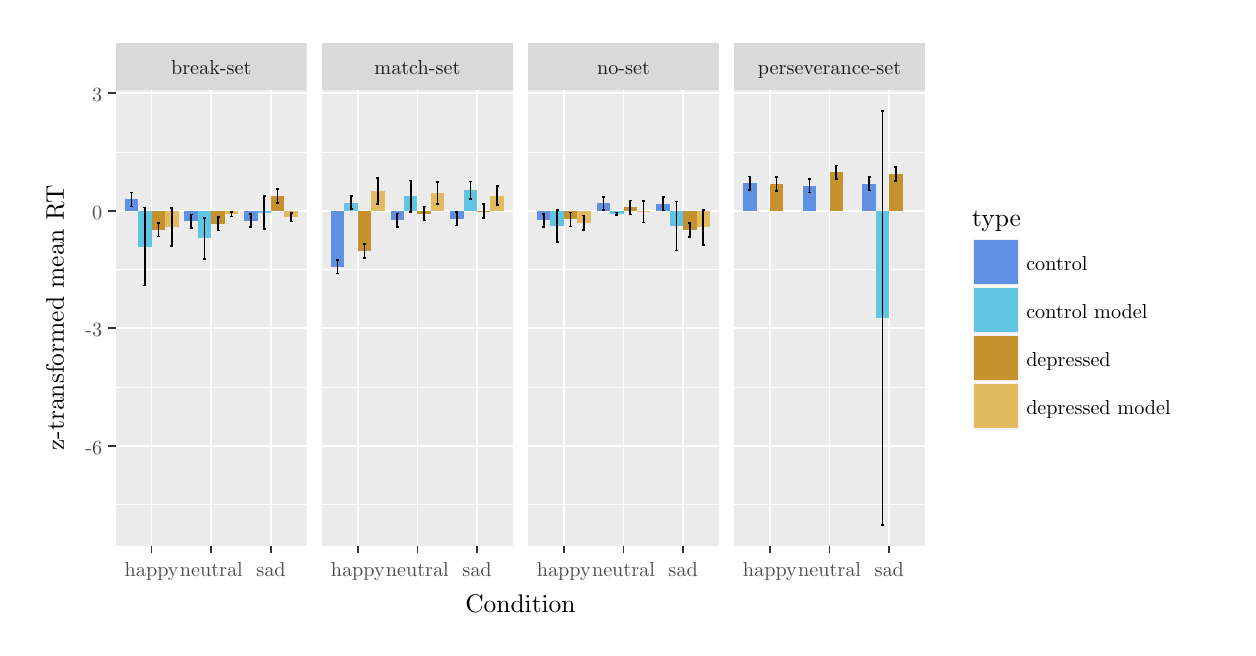
\begin{tikzpicture}[x=1pt,y=1pt]
\definecolor{fillColor}{RGB}{255,255,255}
\path[use as bounding box,fill=fillColor,fill opacity=0.00] (0,0) rectangle (433.62,216.81);
\begin{scope}
\path[clip] (  0.00,  0.00) rectangle (433.62,216.81);
\definecolor{drawColor}{RGB}{255,255,255}
\definecolor{fillColor}{RGB}{255,255,255}

\path[draw=drawColor,line width= 0.6pt,line join=round,line cap=round,fill=fillColor] (  0.00,  0.00) rectangle (433.62,216.81);
\end{scope}
\begin{scope}
\path[clip] ( 31.87, 29.59) rectangle (100.84,194.25);
\definecolor{fillColor}{gray}{0.92}

\path[fill=fillColor] ( 31.87, 29.59) rectangle (100.84,194.25);
\definecolor{drawColor}{RGB}{255,255,255}

\path[draw=drawColor,line width= 0.3pt,line join=round] ( 31.87, 44.45) --
	(100.84, 44.45);

\path[draw=drawColor,line width= 0.3pt,line join=round] ( 31.87, 86.93) --
	(100.84, 86.93);

\path[draw=drawColor,line width= 0.3pt,line join=round] ( 31.87,129.41) --
	(100.84,129.41);

\path[draw=drawColor,line width= 0.3pt,line join=round] ( 31.87,171.89) --
	(100.84,171.89);

\path[draw=drawColor,line width= 0.6pt,line join=round] ( 31.87, 65.69) --
	(100.84, 65.69);

\path[draw=drawColor,line width= 0.6pt,line join=round] ( 31.87,108.17) --
	(100.84,108.17);

\path[draw=drawColor,line width= 0.6pt,line join=round] ( 31.87,150.65) --
	(100.84,150.65);

\path[draw=drawColor,line width= 0.6pt,line join=round] ( 31.87,193.13) --
	(100.84,193.13);

\path[draw=drawColor,line width= 0.6pt,line join=round] ( 44.80, 29.59) --
	( 44.80,194.25);

\path[draw=drawColor,line width= 0.6pt,line join=round] ( 66.36, 29.59) --
	( 66.36,194.25);

\path[draw=drawColor,line width= 0.6pt,line join=round] ( 87.91, 29.59) --
	( 87.91,194.25);
\definecolor{fillColor}{RGB}{226,186,95}

\path[fill=fillColor] ( 49.65,144.78) rectangle ( 54.50,150.65);
\definecolor{fillColor}{RGB}{196,145,45}

\path[fill=fillColor] ( 44.80,143.83) rectangle ( 49.65,150.65);
\definecolor{fillColor}{RGB}{95,197,226}

\path[fill=fillColor] ( 39.95,137.72) rectangle ( 44.80,150.65);
\definecolor{fillColor}{RGB}{95,145,226}

\path[fill=fillColor] ( 35.10,150.65) rectangle ( 39.95,154.72);
\definecolor{fillColor}{RGB}{226,186,95}

\path[fill=fillColor] ( 71.21,149.32) rectangle ( 76.06,150.65);
\definecolor{fillColor}{RGB}{196,145,45}

\path[fill=fillColor] ( 66.36,145.98) rectangle ( 71.21,150.65);
\definecolor{fillColor}{RGB}{95,197,226}

\path[fill=fillColor] ( 61.51,140.67) rectangle ( 66.36,150.65);
\definecolor{fillColor}{RGB}{95,145,226}

\path[fill=fillColor] ( 56.66,146.93) rectangle ( 61.51,150.65);
\definecolor{fillColor}{RGB}{226,186,95}

\path[fill=fillColor] ( 92.76,148.29) rectangle ( 97.61,150.65);
\definecolor{fillColor}{RGB}{196,145,45}

\path[fill=fillColor] ( 87.91,150.65) rectangle ( 92.76,155.91);
\definecolor{fillColor}{RGB}{95,197,226}

\path[fill=fillColor] ( 83.06,149.99) rectangle ( 87.91,150.65);
\definecolor{fillColor}{RGB}{95,145,226}

\path[fill=fillColor] ( 78.21,147.09) rectangle ( 83.06,150.65);
\definecolor{drawColor}{RGB}{0,0,0}

\path[draw=drawColor,line width= 0.6pt,line join=round] ( 51.54,151.72) --
	( 52.62,151.72);

\path[draw=drawColor,line width= 0.6pt,line join=round] ( 52.08,151.72) --
	( 52.08,137.83);

\path[draw=drawColor,line width= 0.6pt,line join=round] ( 51.54,137.83) --
	( 52.62,137.83);

\path[draw=drawColor,line width= 0.6pt,line join=round] ( 46.69,146.34) --
	( 47.77,146.34);

\path[draw=drawColor,line width= 0.6pt,line join=round] ( 47.23,146.34) --
	( 47.23,141.31);

\path[draw=drawColor,line width= 0.6pt,line join=round] ( 46.69,141.31) --
	( 47.77,141.31);

\path[draw=drawColor,line width= 0.6pt,line join=round] ( 41.84,151.81) --
	( 42.92,151.81);

\path[draw=drawColor,line width= 0.6pt,line join=round] ( 42.38,151.81) --
	( 42.38,123.63);

\path[draw=drawColor,line width= 0.6pt,line join=round] ( 41.84,123.63) --
	( 42.92,123.63);

\path[draw=drawColor,line width= 0.6pt,line join=round] ( 36.99,157.20) --
	( 38.07,157.20);

\path[draw=drawColor,line width= 0.6pt,line join=round] ( 37.53,157.20) --
	( 37.53,152.23);

\path[draw=drawColor,line width= 0.6pt,line join=round] ( 36.99,152.23) --
	( 38.07,152.23);

\path[draw=drawColor,line width= 0.6pt,line join=round] ( 73.09,150.10) --
	( 74.17,150.10);

\path[draw=drawColor,line width= 0.6pt,line join=round] ( 73.63,150.10) --
	( 73.63,148.54);

\path[draw=drawColor,line width= 0.6pt,line join=round] ( 73.09,148.54) --
	( 74.17,148.54);

\path[draw=drawColor,line width= 0.6pt,line join=round] ( 68.24,148.48) --
	( 69.32,148.48);

\path[draw=drawColor,line width= 0.6pt,line join=round] ( 68.78,148.48) --
	( 68.78,143.47);

\path[draw=drawColor,line width= 0.6pt,line join=round] ( 68.24,143.47) --
	( 69.32,143.47);

\path[draw=drawColor,line width= 0.6pt,line join=round] ( 63.39,148.04) --
	( 64.47,148.04);

\path[draw=drawColor,line width= 0.6pt,line join=round] ( 63.93,148.04) --
	( 63.93,133.30);

\path[draw=drawColor,line width= 0.6pt,line join=round] ( 63.39,133.30) --
	( 64.47,133.30);

\path[draw=drawColor,line width= 0.6pt,line join=round] ( 58.54,149.34) --
	( 59.62,149.34);

\path[draw=drawColor,line width= 0.6pt,line join=round] ( 59.08,149.34) --
	( 59.08,144.51);

\path[draw=drawColor,line width= 0.6pt,line join=round] ( 58.54,144.51) --
	( 59.62,144.51);

\path[draw=drawColor,line width= 0.6pt,line join=round] ( 94.65,149.86) --
	( 95.72,149.86);

\path[draw=drawColor,line width= 0.6pt,line join=round] ( 95.18,149.86) --
	( 95.18,146.72);

\path[draw=drawColor,line width= 0.6pt,line join=round] ( 94.65,146.72) --
	( 95.72,146.72);

\path[draw=drawColor,line width= 0.6pt,line join=round] ( 89.80,158.42) --
	( 90.87,158.42);

\path[draw=drawColor,line width= 0.6pt,line join=round] ( 90.33,158.42) --
	( 90.33,153.39);

\path[draw=drawColor,line width= 0.6pt,line join=round] ( 89.80,153.39) --
	( 90.87,153.39);

\path[draw=drawColor,line width= 0.6pt,line join=round] ( 84.95,155.96) --
	( 86.02,155.96);

\path[draw=drawColor,line width= 0.6pt,line join=round] ( 85.48,155.96) --
	( 85.48,144.02);

\path[draw=drawColor,line width= 0.6pt,line join=round] ( 84.95,144.02) --
	( 86.02,144.02);

\path[draw=drawColor,line width= 0.6pt,line join=round] ( 80.10,149.50) --
	( 81.17,149.50);

\path[draw=drawColor,line width= 0.6pt,line join=round] ( 80.64,149.50) --
	( 80.64,144.67);

\path[draw=drawColor,line width= 0.6pt,line join=round] ( 80.10,144.67) --
	( 81.17,144.67);
\end{scope}
\begin{scope}
\path[clip] (106.34, 29.59) rectangle (175.31,194.25);
\definecolor{fillColor}{gray}{0.92}

\path[fill=fillColor] (106.34, 29.59) rectangle (175.31,194.25);
\definecolor{drawColor}{RGB}{255,255,255}

\path[draw=drawColor,line width= 0.3pt,line join=round] (106.34, 44.45) --
	(175.31, 44.45);

\path[draw=drawColor,line width= 0.3pt,line join=round] (106.34, 86.93) --
	(175.31, 86.93);

\path[draw=drawColor,line width= 0.3pt,line join=round] (106.34,129.41) --
	(175.31,129.41);

\path[draw=drawColor,line width= 0.3pt,line join=round] (106.34,171.89) --
	(175.31,171.89);

\path[draw=drawColor,line width= 0.6pt,line join=round] (106.34, 65.69) --
	(175.31, 65.69);

\path[draw=drawColor,line width= 0.6pt,line join=round] (106.34,108.17) --
	(175.31,108.17);

\path[draw=drawColor,line width= 0.6pt,line join=round] (106.34,150.65) --
	(175.31,150.65);

\path[draw=drawColor,line width= 0.6pt,line join=round] (106.34,193.13) --
	(175.31,193.13);

\path[draw=drawColor,line width= 0.6pt,line join=round] (119.27, 29.59) --
	(119.27,194.25);

\path[draw=drawColor,line width= 0.6pt,line join=round] (140.83, 29.59) --
	(140.83,194.25);

\path[draw=drawColor,line width= 0.6pt,line join=round] (162.38, 29.59) --
	(162.38,194.25);
\definecolor{fillColor}{RGB}{226,186,95}

\path[fill=fillColor] (124.12,150.65) rectangle (128.97,157.78);
\definecolor{fillColor}{RGB}{196,145,45}

\path[fill=fillColor] (119.27,136.07) rectangle (124.12,150.65);
\definecolor{fillColor}{RGB}{95,197,226}

\path[fill=fillColor] (114.42,150.65) rectangle (119.27,153.63);
\definecolor{fillColor}{RGB}{95,145,226}

\path[fill=fillColor] (109.57,130.43) rectangle (114.42,150.65);
\definecolor{fillColor}{RGB}{226,186,95}

\path[fill=fillColor] (145.68,150.65) rectangle (150.53,157.11);
\definecolor{fillColor}{RGB}{196,145,45}

\path[fill=fillColor] (140.83,149.62) rectangle (145.68,150.65);
\definecolor{fillColor}{RGB}{95,197,226}

\path[fill=fillColor] (135.98,150.65) rectangle (140.83,155.86);
\definecolor{fillColor}{RGB}{95,145,226}

\path[fill=fillColor] (131.13,147.26) rectangle (135.98,150.65);
\definecolor{fillColor}{RGB}{226,186,95}

\path[fill=fillColor] (167.23,150.65) rectangle (172.08,156.13);
\definecolor{fillColor}{RGB}{196,145,45}

\path[fill=fillColor] (162.38,150.60) rectangle (167.23,150.65);
\definecolor{fillColor}{RGB}{95,197,226}

\path[fill=fillColor] (157.53,150.65) rectangle (162.38,158.07);
\definecolor{fillColor}{RGB}{95,145,226}

\path[fill=fillColor] (152.68,147.73) rectangle (157.53,150.65);
\definecolor{drawColor}{RGB}{0,0,0}

\path[draw=drawColor,line width= 0.6pt,line join=round] (126.01,162.43) --
	(127.09,162.43);

\path[draw=drawColor,line width= 0.6pt,line join=round] (126.55,162.43) --
	(126.55,153.13);

\path[draw=drawColor,line width= 0.6pt,line join=round] (126.01,153.13) --
	(127.09,153.13);

\path[draw=drawColor,line width= 0.6pt,line join=round] (121.16,138.57) --
	(122.24,138.57);

\path[draw=drawColor,line width= 0.6pt,line join=round] (121.70,138.57) --
	(121.70,133.56);

\path[draw=drawColor,line width= 0.6pt,line join=round] (121.16,133.56) --
	(122.24,133.56);

\path[draw=drawColor,line width= 0.6pt,line join=round] (116.31,156.06) --
	(117.39,156.06);

\path[draw=drawColor,line width= 0.6pt,line join=round] (116.85,156.06) --
	(116.85,151.21);

\path[draw=drawColor,line width= 0.6pt,line join=round] (116.31,151.21) --
	(117.39,151.21);

\path[draw=drawColor,line width= 0.6pt,line join=round] (111.46,132.85) --
	(112.54,132.85);

\path[draw=drawColor,line width= 0.6pt,line join=round] (112.00,132.85) --
	(112.00,128.00);

\path[draw=drawColor,line width= 0.6pt,line join=round] (111.46,128.00) --
	(112.54,128.00);

\path[draw=drawColor,line width= 0.6pt,line join=round] (147.56,161.07) --
	(148.64,161.07);

\path[draw=drawColor,line width= 0.6pt,line join=round] (148.10,161.07) --
	(148.10,153.15);

\path[draw=drawColor,line width= 0.6pt,line join=round] (147.56,153.15) --
	(148.64,153.15);

\path[draw=drawColor,line width= 0.6pt,line join=round] (142.71,152.13) --
	(143.79,152.13);

\path[draw=drawColor,line width= 0.6pt,line join=round] (143.25,152.13) --
	(143.25,147.12);

\path[draw=drawColor,line width= 0.6pt,line join=round] (142.71,147.12) --
	(143.79,147.12);

\path[draw=drawColor,line width= 0.6pt,line join=round] (137.86,161.55) --
	(138.94,161.55);

\path[draw=drawColor,line width= 0.6pt,line join=round] (138.40,161.55) --
	(138.40,150.17);

\path[draw=drawColor,line width= 0.6pt,line join=round] (137.86,150.17) --
	(138.94,150.17);

\path[draw=drawColor,line width= 0.6pt,line join=round] (133.01,149.68) --
	(134.09,149.68);

\path[draw=drawColor,line width= 0.6pt,line join=round] (133.55,149.68) --
	(133.55,144.85);

\path[draw=drawColor,line width= 0.6pt,line join=round] (133.01,144.85) --
	(134.09,144.85);

\path[draw=drawColor,line width= 0.6pt,line join=round] (169.12,159.57) --
	(170.19,159.57);

\path[draw=drawColor,line width= 0.6pt,line join=round] (169.65,159.57) --
	(169.65,152.68);

\path[draw=drawColor,line width= 0.6pt,line join=round] (169.12,152.68) --
	(170.19,152.68);

\path[draw=drawColor,line width= 0.6pt,line join=round] (164.27,153.11) --
	(165.34,153.11);

\path[draw=drawColor,line width= 0.6pt,line join=round] (164.80,153.11) --
	(164.80,148.10);

\path[draw=drawColor,line width= 0.6pt,line join=round] (164.27,148.10) --
	(165.34,148.10);

\path[draw=drawColor,line width= 0.6pt,line join=round] (159.42,161.28) --
	(160.49,161.28);

\path[draw=drawColor,line width= 0.6pt,line join=round] (159.96,161.28) --
	(159.96,154.86);

\path[draw=drawColor,line width= 0.6pt,line join=round] (159.42,154.86) --
	(160.49,154.86);

\path[draw=drawColor,line width= 0.6pt,line join=round] (154.57,150.15) --
	(155.64,150.15);

\path[draw=drawColor,line width= 0.6pt,line join=round] (155.11,150.15) --
	(155.11,145.31);

\path[draw=drawColor,line width= 0.6pt,line join=round] (154.57,145.31) --
	(155.64,145.31);
\end{scope}
\begin{scope}
\path[clip] (180.81, 29.59) rectangle (249.78,194.25);
\definecolor{fillColor}{gray}{0.92}

\path[fill=fillColor] (180.81, 29.59) rectangle (249.78,194.25);
\definecolor{drawColor}{RGB}{255,255,255}

\path[draw=drawColor,line width= 0.3pt,line join=round] (180.81, 44.45) --
	(249.78, 44.45);

\path[draw=drawColor,line width= 0.3pt,line join=round] (180.81, 86.93) --
	(249.78, 86.93);

\path[draw=drawColor,line width= 0.3pt,line join=round] (180.81,129.41) --
	(249.78,129.41);

\path[draw=drawColor,line width= 0.3pt,line join=round] (180.81,171.89) --
	(249.78,171.89);

\path[draw=drawColor,line width= 0.6pt,line join=round] (180.81, 65.69) --
	(249.78, 65.69);

\path[draw=drawColor,line width= 0.6pt,line join=round] (180.81,108.17) --
	(249.78,108.17);

\path[draw=drawColor,line width= 0.6pt,line join=round] (180.81,150.65) --
	(249.78,150.65);

\path[draw=drawColor,line width= 0.6pt,line join=round] (180.81,193.13) --
	(249.78,193.13);

\path[draw=drawColor,line width= 0.6pt,line join=round] (193.74, 29.59) --
	(193.74,194.25);

\path[draw=drawColor,line width= 0.6pt,line join=round] (215.30, 29.59) --
	(215.30,194.25);

\path[draw=drawColor,line width= 0.6pt,line join=round] (236.85, 29.59) --
	(236.85,194.25);
\definecolor{fillColor}{RGB}{226,186,95}

\path[fill=fillColor] (198.59,146.31) rectangle (203.44,150.65);
\definecolor{fillColor}{RGB}{196,145,45}

\path[fill=fillColor] (193.74,147.50) rectangle (198.59,150.65);
\definecolor{fillColor}{RGB}{95,197,226}

\path[fill=fillColor] (188.89,145.25) rectangle (193.74,150.65);
\definecolor{fillColor}{RGB}{95,145,226}

\path[fill=fillColor] (184.05,147.13) rectangle (188.89,150.65);
\definecolor{fillColor}{RGB}{226,186,95}

\path[fill=fillColor] (220.15,150.30) rectangle (225.00,150.65);
\definecolor{fillColor}{RGB}{196,145,45}

\path[fill=fillColor] (215.30,150.65) rectangle (220.15,151.84);
\definecolor{fillColor}{RGB}{95,197,226}

\path[fill=fillColor] (210.45,149.52) rectangle (215.30,150.65);
\definecolor{fillColor}{RGB}{95,145,226}

\path[fill=fillColor] (205.60,150.65) rectangle (210.45,153.32);
\definecolor{fillColor}{RGB}{226,186,95}

\path[fill=fillColor] (241.70,144.70) rectangle (246.55,150.65);
\definecolor{fillColor}{RGB}{196,145,45}

\path[fill=fillColor] (236.85,143.78) rectangle (241.70,150.65);
\definecolor{fillColor}{RGB}{95,197,226}

\path[fill=fillColor] (232.00,145.11) rectangle (236.85,150.65);
\definecolor{fillColor}{RGB}{95,145,226}

\path[fill=fillColor] (227.15,150.65) rectangle (232.00,153.11);
\definecolor{drawColor}{RGB}{0,0,0}

\path[draw=drawColor,line width= 0.6pt,line join=round] (200.48,148.92) --
	(201.56,148.92);

\path[draw=drawColor,line width= 0.6pt,line join=round] (201.02,148.92) --
	(201.02,143.69);

\path[draw=drawColor,line width= 0.6pt,line join=round] (200.48,143.69) --
	(201.56,143.69);

\path[draw=drawColor,line width= 0.6pt,line join=round] (195.63,150.01) --
	(196.71,150.01);

\path[draw=drawColor,line width= 0.6pt,line join=round] (196.17,150.01) --
	(196.17,145.00);

\path[draw=drawColor,line width= 0.6pt,line join=round] (195.63,145.00) --
	(196.71,145.00);

\path[draw=drawColor,line width= 0.6pt,line join=round] (190.78,151.03) --
	(191.86,151.03);

\path[draw=drawColor,line width= 0.6pt,line join=round] (191.32,151.03) --
	(191.32,139.48);

\path[draw=drawColor,line width= 0.6pt,line join=round] (190.78,139.48) --
	(191.86,139.48);

\path[draw=drawColor,line width= 0.6pt,line join=round] (185.93,149.56) --
	(187.01,149.56);

\path[draw=drawColor,line width= 0.6pt,line join=round] (186.47,149.56) --
	(186.47,144.71);

\path[draw=drawColor,line width= 0.6pt,line join=round] (185.93,144.71) --
	(187.01,144.71);

\path[draw=drawColor,line width= 0.6pt,line join=round] (222.03,154.14) --
	(223.11,154.14);

\path[draw=drawColor,line width= 0.6pt,line join=round] (222.57,154.14) --
	(222.57,146.46);

\path[draw=drawColor,line width= 0.6pt,line join=round] (222.03,146.46) --
	(223.11,146.46);

\path[draw=drawColor,line width= 0.6pt,line join=round] (217.18,154.36) --
	(218.26,154.36);

\path[draw=drawColor,line width= 0.6pt,line join=round] (217.72,154.36) --
	(217.72,149.33);

\path[draw=drawColor,line width= 0.6pt,line join=round] (217.18,149.33) --
	(218.26,149.33);

\path[draw=drawColor,line width= 0.6pt,line join=round] (212.33,150.02) --
	(213.41,150.02);

\path[draw=drawColor,line width= 0.6pt,line join=round] (212.87,150.02) --
	(212.87,149.03);

\path[draw=drawColor,line width= 0.6pt,line join=round] (212.33,149.03) --
	(213.41,149.03);

\path[draw=drawColor,line width= 0.6pt,line join=round] (207.48,155.74) --
	(208.56,155.74);

\path[draw=drawColor,line width= 0.6pt,line join=round] (208.02,155.74) --
	(208.02,150.90);

\path[draw=drawColor,line width= 0.6pt,line join=round] (207.48,150.90) --
	(208.56,150.90);

\path[draw=drawColor,line width= 0.6pt,line join=round] (243.59,151.04) --
	(244.66,151.04);

\path[draw=drawColor,line width= 0.6pt,line join=round] (244.12,151.04) --
	(244.12,138.36);

\path[draw=drawColor,line width= 0.6pt,line join=round] (243.59,138.36) --
	(244.66,138.36);

\path[draw=drawColor,line width= 0.6pt,line join=round] (238.74,146.28) --
	(239.81,146.28);

\path[draw=drawColor,line width= 0.6pt,line join=round] (239.28,146.28) --
	(239.28,141.27);

\path[draw=drawColor,line width= 0.6pt,line join=round] (238.74,141.27) --
	(239.81,141.27);

\path[draw=drawColor,line width= 0.6pt,line join=round] (233.89,153.98) --
	(234.96,153.98);

\path[draw=drawColor,line width= 0.6pt,line join=round] (234.43,153.98) --
	(234.43,136.24);

\path[draw=drawColor,line width= 0.6pt,line join=round] (233.89,136.24) --
	(234.96,136.24);

\path[draw=drawColor,line width= 0.6pt,line join=round] (229.04,155.53) --
	(230.12,155.53);

\path[draw=drawColor,line width= 0.6pt,line join=round] (229.58,155.53) --
	(229.58,150.69);

\path[draw=drawColor,line width= 0.6pt,line join=round] (229.04,150.69) --
	(230.12,150.69);
\end{scope}
\begin{scope}
\path[clip] (255.28, 29.59) rectangle (324.25,194.25);
\definecolor{fillColor}{gray}{0.92}

\path[fill=fillColor] (255.28, 29.59) rectangle (324.25,194.25);
\definecolor{drawColor}{RGB}{255,255,255}

\path[draw=drawColor,line width= 0.3pt,line join=round] (255.28, 44.45) --
	(324.25, 44.45);

\path[draw=drawColor,line width= 0.3pt,line join=round] (255.28, 86.93) --
	(324.25, 86.93);

\path[draw=drawColor,line width= 0.3pt,line join=round] (255.28,129.41) --
	(324.25,129.41);

\path[draw=drawColor,line width= 0.3pt,line join=round] (255.28,171.89) --
	(324.25,171.89);

\path[draw=drawColor,line width= 0.6pt,line join=round] (255.28, 65.69) --
	(324.25, 65.69);

\path[draw=drawColor,line width= 0.6pt,line join=round] (255.28,108.17) --
	(324.25,108.17);

\path[draw=drawColor,line width= 0.6pt,line join=round] (255.28,150.65) --
	(324.25,150.65);

\path[draw=drawColor,line width= 0.6pt,line join=round] (255.28,193.13) --
	(324.25,193.13);

\path[draw=drawColor,line width= 0.6pt,line join=round] (268.21, 29.59) --
	(268.21,194.25);

\path[draw=drawColor,line width= 0.6pt,line join=round] (289.77, 29.59) --
	(289.77,194.25);

\path[draw=drawColor,line width= 0.6pt,line join=round] (311.32, 29.59) --
	(311.32,194.25);
\definecolor{fillColor}{RGB}{196,145,45}

\path[fill=fillColor] (268.21,150.65) rectangle (273.06,160.31);
\definecolor{fillColor}{RGB}{95,145,226}

\path[fill=fillColor] (258.52,150.65) rectangle (263.37,160.61);
\definecolor{fillColor}{RGB}{196,145,45}

\path[fill=fillColor] (289.77,150.65) rectangle (294.62,164.55);
\definecolor{fillColor}{RGB}{95,145,226}

\path[fill=fillColor] (280.07,150.65) rectangle (284.92,159.63);
\definecolor{fillColor}{RGB}{196,145,45}

\path[fill=fillColor] (311.32,150.65) rectangle (316.17,164.00);
\definecolor{fillColor}{RGB}{95,197,226}

\path[fill=fillColor] (306.47,111.92) rectangle (311.32,150.65);
\definecolor{fillColor}{RGB}{95,145,226}

\path[fill=fillColor] (301.62,150.65) rectangle (306.47,160.44);
\definecolor{drawColor}{RGB}{0,0,0}

\path[draw=drawColor,line width= 0.6pt,line join=round] (270.10,162.81) --
	(271.18,162.81);

\path[draw=drawColor,line width= 0.6pt,line join=round] (270.64,162.81) --
	(270.64,157.80);

\path[draw=drawColor,line width= 0.6pt,line join=round] (270.10,157.80) --
	(271.18,157.80);

\path[draw=drawColor,line width= 0.6pt,line join=round] (260.40,163.03) --
	(261.48,163.03);

\path[draw=drawColor,line width= 0.6pt,line join=round] (260.94,163.03) --
	(260.94,158.19);

\path[draw=drawColor,line width= 0.6pt,line join=round] (260.40,158.19) --
	(261.48,158.19);

\path[draw=drawColor,line width= 0.6pt,line join=round] (291.65,167.05) --
	(292.73,167.05);

\path[draw=drawColor,line width= 0.6pt,line join=round] (292.19,167.05) --
	(292.19,162.04);

\path[draw=drawColor,line width= 0.6pt,line join=round] (291.65,162.04) --
	(292.73,162.04);

\path[draw=drawColor,line width= 0.6pt,line join=round] (281.95,162.05) --
	(283.03,162.05);

\path[draw=drawColor,line width= 0.6pt,line join=round] (282.49,162.05) --
	(282.49,157.22);

\path[draw=drawColor,line width= 0.6pt,line join=round] (281.95,157.22) --
	(283.03,157.22);

\path[draw=drawColor,line width= 0.6pt,line join=round] (313.21,166.51) --
	(314.28,166.51);

\path[draw=drawColor,line width= 0.6pt,line join=round] (313.75,166.51) --
	(313.75,161.50);

\path[draw=drawColor,line width= 0.6pt,line join=round] (313.21,161.50) --
	(314.28,161.50);

\path[draw=drawColor,line width= 0.6pt,line join=round] (308.36,186.76) --
	(309.44,186.76);

\path[draw=drawColor,line width= 0.6pt,line join=round] (308.90,186.76) --
	(308.90, 37.07);

\path[draw=drawColor,line width= 0.6pt,line join=round] (308.36, 37.07) --
	(309.44, 37.07);

\path[draw=drawColor,line width= 0.6pt,line join=round] (303.51,162.85) --
	(304.59,162.85);

\path[draw=drawColor,line width= 0.6pt,line join=round] (304.05,162.85) --
	(304.05,158.02);

\path[draw=drawColor,line width= 0.6pt,line join=round] (303.51,158.02) --
	(304.59,158.02);
\end{scope}
\begin{scope}
\path[clip] ( 31.87,194.25) rectangle (100.84,211.31);
\definecolor{fillColor}{gray}{0.85}

\path[fill=fillColor] ( 31.87,194.25) rectangle (100.84,211.31);
\definecolor{drawColor}{gray}{0.10}

\node[text=drawColor,anchor=base,inner sep=0pt, outer sep=0pt, scale=  0.73] at ( 66.36,199.75) {break-set};
\end{scope}
\begin{scope}
\path[clip] (106.34,194.25) rectangle (175.31,211.31);
\definecolor{fillColor}{gray}{0.85}

\path[fill=fillColor] (106.34,194.25) rectangle (175.31,211.31);
\definecolor{drawColor}{gray}{0.10}

\node[text=drawColor,anchor=base,inner sep=0pt, outer sep=0pt, scale=  0.73] at (140.83,199.75) {match-set};
\end{scope}
\begin{scope}
\path[clip] (180.81,194.25) rectangle (249.78,211.31);
\definecolor{fillColor}{gray}{0.85}

\path[fill=fillColor] (180.81,194.25) rectangle (249.78,211.31);
\definecolor{drawColor}{gray}{0.10}

\node[text=drawColor,anchor=base,inner sep=0pt, outer sep=0pt, scale=  0.73] at (215.30,199.75) {no-set};
\end{scope}
\begin{scope}
\path[clip] (255.28,194.25) rectangle (324.25,211.31);
\definecolor{fillColor}{gray}{0.85}

\path[fill=fillColor] (255.28,194.25) rectangle (324.25,211.31);
\definecolor{drawColor}{gray}{0.10}

\node[text=drawColor,anchor=base,inner sep=0pt, outer sep=0pt, scale=  0.73] at (289.77,199.75) {perseverance-set};
\end{scope}
\begin{scope}
\path[clip] (  0.00,  0.00) rectangle (433.62,216.81);
\definecolor{drawColor}{gray}{0.20}

\path[draw=drawColor,line width= 0.6pt,line join=round] ( 44.80, 26.84) --
	( 44.80, 29.59);

\path[draw=drawColor,line width= 0.6pt,line join=round] ( 66.36, 26.84) --
	( 66.36, 29.59);

\path[draw=drawColor,line width= 0.6pt,line join=round] ( 87.91, 26.84) --
	( 87.91, 29.59);
\end{scope}
\begin{scope}
\path[clip] (  0.00,  0.00) rectangle (433.62,216.81);
\definecolor{drawColor}{gray}{0.30}

\node[text=drawColor,anchor=base,inner sep=0pt, outer sep=0pt, scale=  0.73] at ( 44.80, 18.58) {happy};

\node[text=drawColor,anchor=base,inner sep=0pt, outer sep=0pt, scale=  0.73] at ( 66.36, 18.58) {neutral};

\node[text=drawColor,anchor=base,inner sep=0pt, outer sep=0pt, scale=  0.73] at ( 87.91, 18.58) {sad};
\end{scope}
\begin{scope}
\path[clip] (  0.00,  0.00) rectangle (433.62,216.81);
\definecolor{drawColor}{gray}{0.20}

\path[draw=drawColor,line width= 0.6pt,line join=round] (119.27, 26.84) --
	(119.27, 29.59);

\path[draw=drawColor,line width= 0.6pt,line join=round] (140.83, 26.84) --
	(140.83, 29.59);

\path[draw=drawColor,line width= 0.6pt,line join=round] (162.38, 26.84) --
	(162.38, 29.59);
\end{scope}
\begin{scope}
\path[clip] (  0.00,  0.00) rectangle (433.62,216.81);
\definecolor{drawColor}{gray}{0.30}

\node[text=drawColor,anchor=base,inner sep=0pt, outer sep=0pt, scale=  0.73] at (119.27, 18.58) {happy};

\node[text=drawColor,anchor=base,inner sep=0pt, outer sep=0pt, scale=  0.73] at (140.83, 18.58) {neutral};

\node[text=drawColor,anchor=base,inner sep=0pt, outer sep=0pt, scale=  0.73] at (162.38, 18.58) {sad};
\end{scope}
\begin{scope}
\path[clip] (  0.00,  0.00) rectangle (433.62,216.81);
\definecolor{drawColor}{gray}{0.20}

\path[draw=drawColor,line width= 0.6pt,line join=round] (193.74, 26.84) --
	(193.74, 29.59);

\path[draw=drawColor,line width= 0.6pt,line join=round] (215.30, 26.84) --
	(215.30, 29.59);

\path[draw=drawColor,line width= 0.6pt,line join=round] (236.85, 26.84) --
	(236.85, 29.59);
\end{scope}
\begin{scope}
\path[clip] (  0.00,  0.00) rectangle (433.62,216.81);
\definecolor{drawColor}{gray}{0.30}

\node[text=drawColor,anchor=base,inner sep=0pt, outer sep=0pt, scale=  0.73] at (193.74, 18.58) {happy};

\node[text=drawColor,anchor=base,inner sep=0pt, outer sep=0pt, scale=  0.73] at (215.30, 18.58) {neutral};

\node[text=drawColor,anchor=base,inner sep=0pt, outer sep=0pt, scale=  0.73] at (236.85, 18.58) {sad};
\end{scope}
\begin{scope}
\path[clip] (  0.00,  0.00) rectangle (433.62,216.81);
\definecolor{drawColor}{gray}{0.20}

\path[draw=drawColor,line width= 0.6pt,line join=round] (268.21, 26.84) --
	(268.21, 29.59);

\path[draw=drawColor,line width= 0.6pt,line join=round] (289.77, 26.84) --
	(289.77, 29.59);

\path[draw=drawColor,line width= 0.6pt,line join=round] (311.32, 26.84) --
	(311.32, 29.59);
\end{scope}
\begin{scope}
\path[clip] (  0.00,  0.00) rectangle (433.62,216.81);
\definecolor{drawColor}{gray}{0.30}

\node[text=drawColor,anchor=base,inner sep=0pt, outer sep=0pt, scale=  0.73] at (268.21, 18.58) {happy};

\node[text=drawColor,anchor=base,inner sep=0pt, outer sep=0pt, scale=  0.73] at (289.77, 18.58) {neutral};

\node[text=drawColor,anchor=base,inner sep=0pt, outer sep=0pt, scale=  0.73] at (311.32, 18.58) {sad};
\end{scope}
\begin{scope}
\path[clip] (  0.00,  0.00) rectangle (433.62,216.81);
\definecolor{drawColor}{gray}{0.30}

\node[text=drawColor,anchor=base east,inner sep=0pt, outer sep=0pt, scale=  0.73] at ( 26.92, 62.66) {-6};

\node[text=drawColor,anchor=base east,inner sep=0pt, outer sep=0pt, scale=  0.73] at ( 26.92,105.14) {-3};

\node[text=drawColor,anchor=base east,inner sep=0pt, outer sep=0pt, scale=  0.73] at ( 26.92,147.62) {0};

\node[text=drawColor,anchor=base east,inner sep=0pt, outer sep=0pt, scale=  0.73] at ( 26.92,190.10) {3};
\end{scope}
\begin{scope}
\path[clip] (  0.00,  0.00) rectangle (433.62,216.81);
\definecolor{drawColor}{gray}{0.20}

\path[draw=drawColor,line width= 0.6pt,line join=round] ( 29.12, 65.69) --
	( 31.87, 65.69);

\path[draw=drawColor,line width= 0.6pt,line join=round] ( 29.12,108.17) --
	( 31.87,108.17);

\path[draw=drawColor,line width= 0.6pt,line join=round] ( 29.12,150.65) --
	( 31.87,150.65);

\path[draw=drawColor,line width= 0.6pt,line join=round] ( 29.12,193.13) --
	( 31.87,193.13);
\end{scope}
\begin{scope}
\path[clip] (  0.00,  0.00) rectangle (433.62,216.81);
\definecolor{drawColor}{RGB}{0,0,0}

\node[text=drawColor,anchor=base,inner sep=0pt, outer sep=0pt, scale=  0.92] at (178.06,  5.50) {Condition};
\end{scope}
\begin{scope}
\path[clip] (  0.00,  0.00) rectangle (433.62,216.81);
\definecolor{drawColor}{RGB}{0,0,0}

\node[text=drawColor,rotate= 90.00,anchor=base,inner sep=0pt, outer sep=0pt, scale=  0.92] at ( 13.08,111.92) {z-transformed mean RT};
\end{scope}
\begin{scope}
\path[clip] (  0.00,  0.00) rectangle (433.62,216.81);
\definecolor{fillColor}{RGB}{255,255,255}

\path[fill=fillColor] (335.63, 65.58) rectangle (428.12,158.25);
\end{scope}
\begin{scope}
\path[clip] (  0.00,  0.00) rectangle (433.62,216.81);
\definecolor{drawColor}{RGB}{0,0,0}

\node[text=drawColor,anchor=base west,inner sep=0pt, outer sep=0pt, scale=  0.92] at (341.32,144.99) {type};
\end{scope}
\begin{scope}
\path[clip] (  0.00,  0.00) rectangle (433.62,216.81);
\definecolor{drawColor}{RGB}{255,255,255}
\definecolor{fillColor}{gray}{0.95}

\path[draw=drawColor,line width= 0.6pt,line join=round,line cap=round,fill=fillColor] (341.32,123.31) rectangle (358.67,140.65);
\end{scope}
\begin{scope}
\path[clip] (  0.00,  0.00) rectangle (433.62,216.81);
\definecolor{fillColor}{RGB}{95,145,226}

\path[fill=fillColor] (342.04,124.02) rectangle (357.96,139.94);
\end{scope}
\begin{scope}
\path[clip] (  0.00,  0.00) rectangle (433.62,216.81);
\definecolor{drawColor}{RGB}{255,255,255}
\definecolor{fillColor}{gray}{0.95}

\path[draw=drawColor,line width= 0.6pt,line join=round,line cap=round,fill=fillColor] (341.32,105.96) rectangle (358.67,123.31);
\end{scope}
\begin{scope}
\path[clip] (  0.00,  0.00) rectangle (433.62,216.81);
\definecolor{fillColor}{RGB}{95,197,226}

\path[fill=fillColor] (342.04,106.67) rectangle (357.96,122.60);
\end{scope}
\begin{scope}
\path[clip] (  0.00,  0.00) rectangle (433.62,216.81);
\definecolor{drawColor}{RGB}{255,255,255}
\definecolor{fillColor}{gray}{0.95}

\path[draw=drawColor,line width= 0.6pt,line join=round,line cap=round,fill=fillColor] (341.32, 88.62) rectangle (358.67,105.96);
\end{scope}
\begin{scope}
\path[clip] (  0.00,  0.00) rectangle (433.62,216.81);
\definecolor{fillColor}{RGB}{196,145,45}

\path[fill=fillColor] (342.04, 89.33) rectangle (357.96,105.25);
\end{scope}
\begin{scope}
\path[clip] (  0.00,  0.00) rectangle (433.62,216.81);
\definecolor{drawColor}{RGB}{255,255,255}
\definecolor{fillColor}{gray}{0.95}

\path[draw=drawColor,line width= 0.6pt,line join=round,line cap=round,fill=fillColor] (341.32, 71.27) rectangle (358.67, 88.62);
\end{scope}
\begin{scope}
\path[clip] (  0.00,  0.00) rectangle (433.62,216.81);
\definecolor{fillColor}{RGB}{226,186,95}

\path[fill=fillColor] (342.04, 71.98) rectangle (357.96, 87.91);
\end{scope}
\begin{scope}
\path[clip] (  0.00,  0.00) rectangle (433.62,216.81);
\definecolor{drawColor}{RGB}{0,0,0}

\node[text=drawColor,anchor=base west,inner sep=0pt, outer sep=0pt, scale=  0.73] at (360.84,128.95) {control};
\end{scope}
\begin{scope}
\path[clip] (  0.00,  0.00) rectangle (433.62,216.81);
\definecolor{drawColor}{RGB}{0,0,0}

\node[text=drawColor,anchor=base west,inner sep=0pt, outer sep=0pt, scale=  0.73] at (360.84,111.60) {control model};
\end{scope}
\begin{scope}
\path[clip] (  0.00,  0.00) rectangle (433.62,216.81);
\definecolor{drawColor}{RGB}{0,0,0}

\node[text=drawColor,anchor=base west,inner sep=0pt, outer sep=0pt, scale=  0.73] at (360.84, 94.26) {depressed};
\end{scope}
\begin{scope}
\path[clip] (  0.00,  0.00) rectangle (433.62,216.81);
\definecolor{drawColor}{RGB}{0,0,0}

\node[text=drawColor,anchor=base west,inner sep=0pt, outer sep=0pt, scale=  0.73] at (360.84, 76.91) {depressed model};
\end{scope}
\end{tikzpicture}
